\section{ATLAS Detector}
\label{sec:ATLAS}

A Toroidal LHC ApparatuS (ATLAS) is a general-purpose detector of LHC that detects events from proton-proton, and heavy ion collisions \cite{ATLAS}. It is a $44$ meters long and $25$ meters wide cylindrical-shaped detector built around LHC Interaction Point 1 \cite{ATLAS}. ATLAS has multiple concentric sub-detectors layered around the beamline, providing forward-backward symmetric coverage. The two proton beams collide at the center of the detector producing outgoing particles from hard scattering, underlying events, and pile-up. The outgoing particles interact with the detector material leaving tracks and energy deposits in several layers of the sub-detectors. The sub-detector closest to the beamline is called \textit{Inner Detector (ID)}, which measures the trajectories of the charged particle and plays a crucial role in identifying the physical position of hard-scattering, also known as the \textit{interaction point (IP)}. ID is surrounded by a solenoid magnet that provides a $2$ Tesla magnetic field to bend the particle trajectories for momentum measurements \cite{ATLAS}. After the solenoid magnet lies the \textit{electromagnetic calorimeter (ECAL)} and then the \textit{hadronic calorimeter (HCAL)}, which measure the energy of electromagnetic and hadronic physic objects, respectively. The outermost layer of the ATLAS detector is the \textit{Muon Spectrometer(MS)} that provides a secondary measure of muon trajectories for momentum measurement. MS is embedded inside a toroidal magnetic field that provides a magnetic field up to 3.5 Tesla \cite{ATLAS}. Figure \ref{fig:ATLAS} shows a schematic of the ATLAS detector with all its sub-detectors.

\begin{figure}
    \centering
    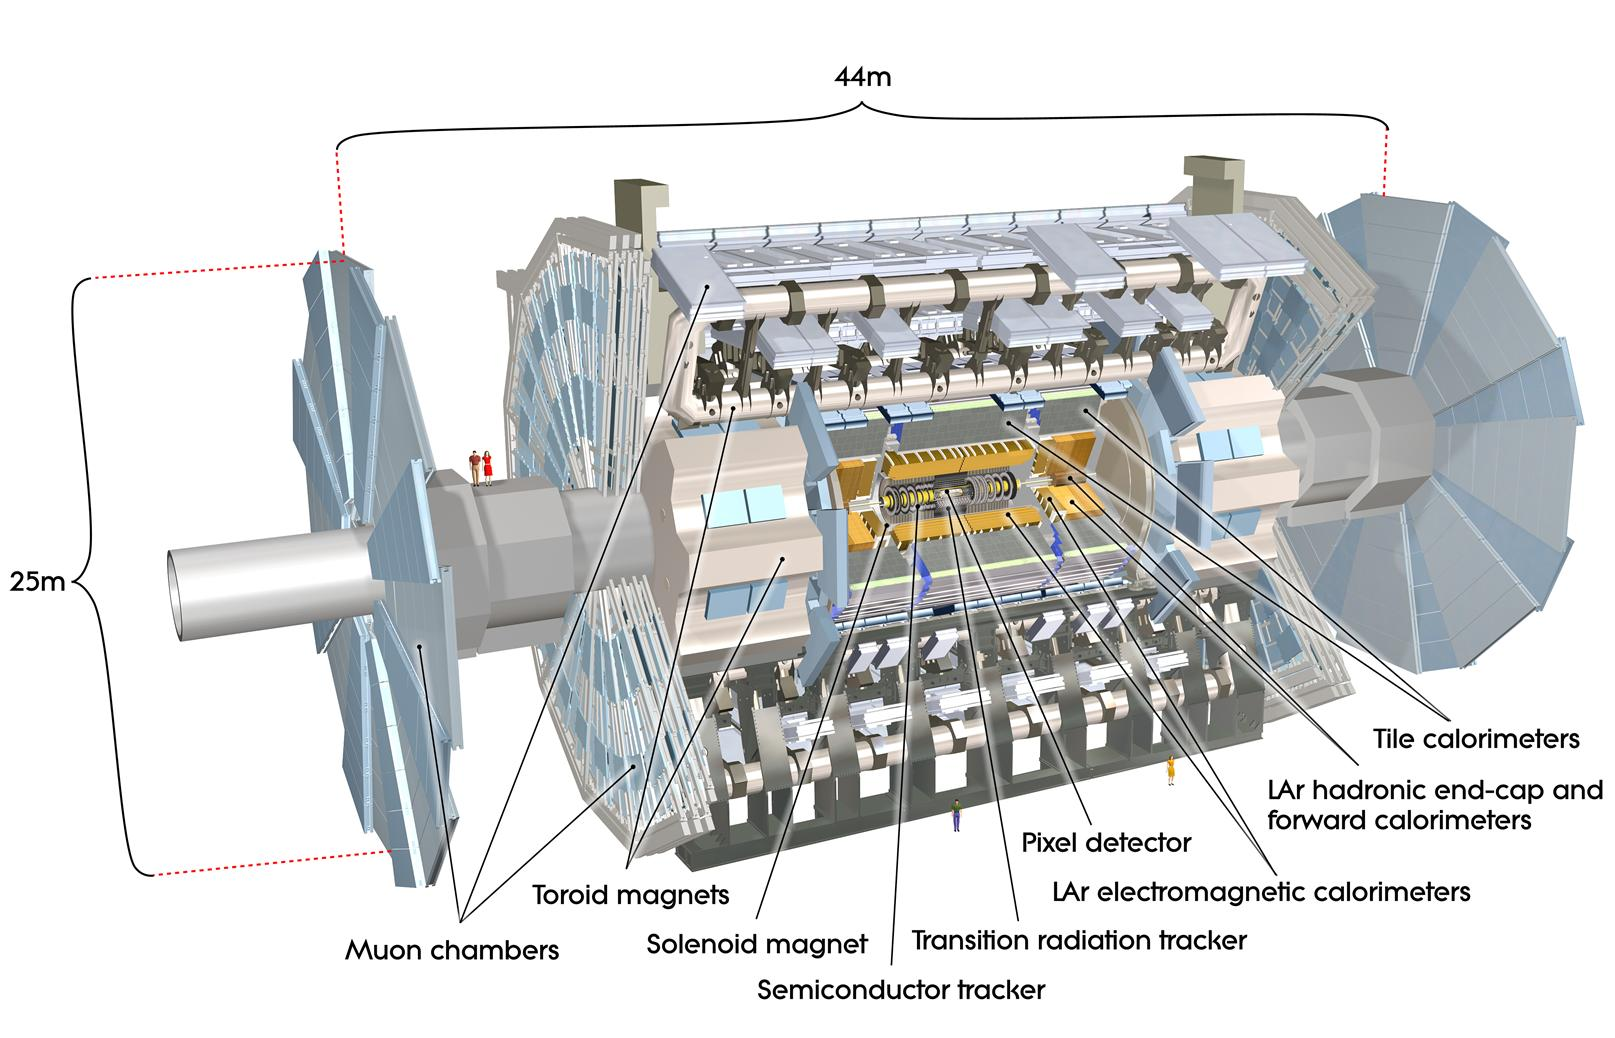
\includegraphics[width=.98\linewidth]{figures/LHC/AtlasDetector.png}
    \caption{ A detailed schematic of the ATLAS detector with all its sub-detectors \cite{ATLAS}.\label{fig:ATLAS}}
\end{figure}

\subsection{ATLAS Coordinate System}
\label{subsec:ATLASCS}

ATLAS measurements use a right-handed coordinate system with the nominal interaction point as the origin. The beamline is along the cylindrical axis of symmetry of the detector, which defines the longitudinal \textit{z}-axis. The transverse \textit{xy}-plane is perpendicular to the beam direction, where \textit{x}-axis points to the center of the LHC ring and \textit{y}-axis points upwards towards the surface. Figure \ref{fig:ATLAS_CS} shows a schematic of the ATLAS coordinate system. The angle measured around the beamline in \textit{xy}-plane gives the azimuthal angle $\phi$, whereas the angle measured with respect to the \textit{z}-axis gives the polar angle $\theta$. Transverse momentum ($p_{T}$) is particle's momentum in the \textit{xy}-plane, defined as, 

\begin{equation}
p_{T} = \sqrt{p_{x}^2+p_{y}^2}=p\sin\theta
\label{eqn:pT}
\end{equation}
\begin{figure}
    \centering
    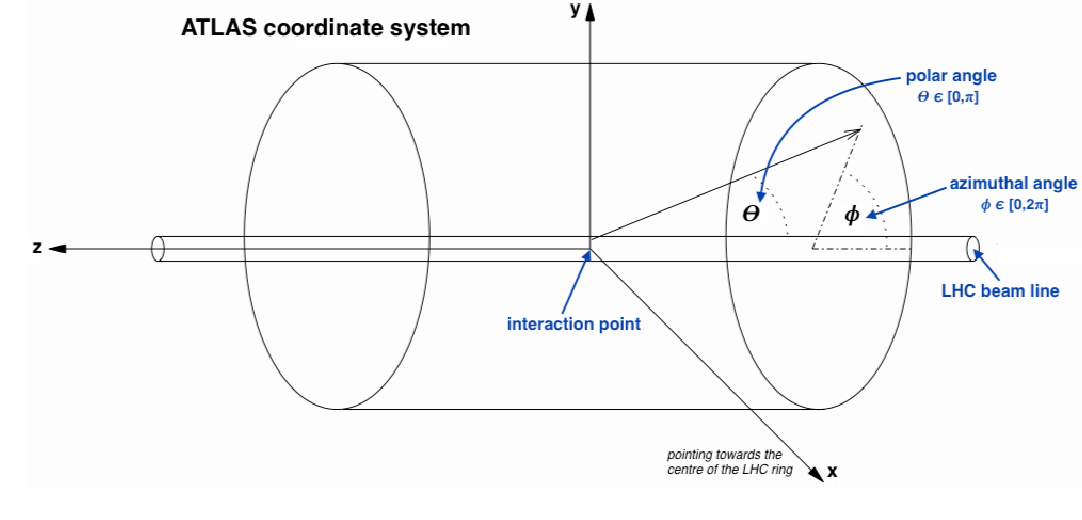
\includegraphics[width=.98\linewidth]{figures/LHC/ATLAS_CoordinateSys.png}
    \caption{ A schematic of the right-handed ATLAS coordinate system \cite{ATLAS_CoordSys}.\label{fig:ATLAS_CS}}
\end{figure}

\textit{Rapidity (y)} defined in terms of a particle's energy ($E$) and momentum ($p$) is a commonly used collider physics quantity that measures whether an outgoing particle is produced perpendicular or parallel to the \textit{z}-axis. Rapidity is defined as, 

\begin{equation}
    y = \frac{1}{2}\ln{ \left( \frac{E+p_{z}}{E-p_{z}} \right) }
    \label{eqn:Rapidity}
\end{equation}
Particles with larger momentum along the \textit{z}-axis have larger values of rapidity, whereas particles with larger momentum values in the transverse plane have smaller values of rapidity. For particles with negligible mass, the rapidity approaches a purely angular variable called \textit{pseudorapidity ($\eta$)} defined as, 

\begin{equation}
    \eta = \frac{1}{2}\ln{ \left( \frac{ |\vec{p}|+p_{z}}{ |\vec{p}| -p_{z}} \right) } = -ln { \left[ \tan \left( \frac{\theta}{2}\right) \right] } 
    \label{eqn:PseudoRapidity}
\end{equation}
Higher values of rapidity and pseudorapidity refer to the forward region of the detector. ATLAS detector has full $2\pi$ coverage in $\phi$ and maximum coverage of $|\eta| < 4.5$ corresponding to $1.3^{\circ} < \theta < 178.7^{\circ} $ \cite{ATLAS}. 

\subsection{Inner Detector}
\label{subsec:ID}
The inner detector is the innermost sub-detector of ATLAS and is responsible for tracking charged particles' trajectories and identifying the interaction point of the hard scatter. Closest to the interaction point is the Insertable B-Layer (IBL) \cite{ATLAS_IBL}, which was installed during the long-upgrade shutdown between Run-1 and Run-2 to maintain the tracking requirements at higher pile-up. The IBL is highly granular, consisting of roughly 12 million silicon pixel sensors with a size of $50\times 250 ~\mu m^2$ \cite{ATLAS_IBL}. IBL is located $3.3$ cm from the beamline and can reconstruct tracks within the pseudorapidity range of $|\eta|<2.5$ \cite{ATLAS_IBL}. 

Three layers of silicon-pixel detectors with $1,744$ pixel sensors, each comprising $47,232$ pixels of size $50\times 400 ~\mu m^2$ surround the IBL \cite{ID_Pixel}. The slightly larger pixel size is adequate for the pile-up at a distance larger than $5$ cm from the interaction point. These pixel layers were also present during the Run-1 data-taking period and provided coverage up to $|\eta|<2.5$ with a spatial resolution between $5$ and 12 $\mu$m \cite{ID_Pixel}. Surrounding the pixel layers is the Semiconductor Tracker (SCT) consisting of five layers of silicon microstrip detectors with a mean strip pitch of $80 ~\mu m$ in the barrel region and varying pitch of  $57-94 ~\mu m$ in the end-cap region \cite{ID_Strips}. 

At a distance about $50$ cm from the beamline lies the outermost layer of the ATLAS inner detector, the Transition Radiation Tracker (TRT), with $370,000$ straw tubes with a diameter of $4$ mm \cite{ID_TRT}. Each TRT straw tube is filled with a Xenon-based gas mixture and consists of $31~\mu m$ diameter tungsten wires \cite{ID_TRT}. A charged particle passing through different layers of ID leaves a track via ionization. 

Figure \ref{fig:ATLAS_ID} schematically shows different parts of the inner detector and their distances from the interaction point.

\begin{figure}
    \centering
    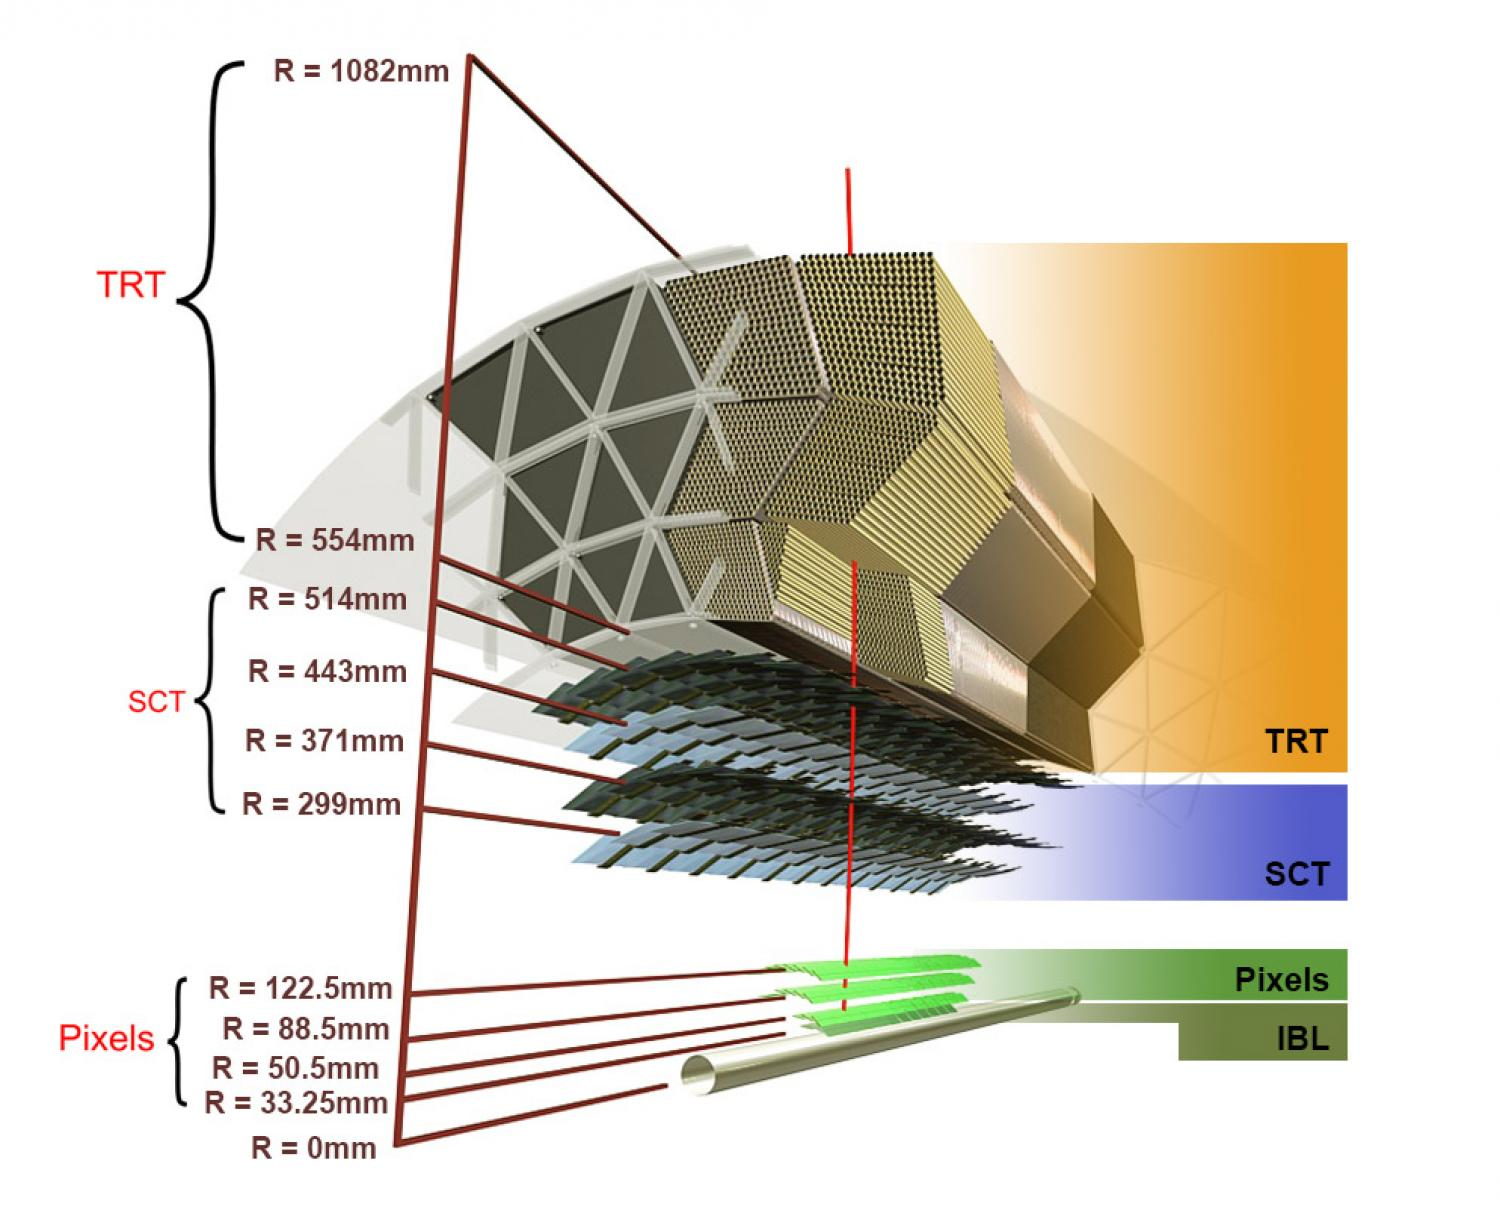
\includegraphics[width=.98\linewidth]{figures/LHC/ATLAS_InnerDetector.jpg}
    \caption{ A schematic of the inner detector of ATLAS showing the IBL pixel detectors, SCT, and TRT \cite{ID_Align_Run2}.\label{fig:ATLAS_ID}}
\end{figure}

\subsection{Calorimeters}
\label{subsec:Cal}

ATLAS has two calorimeters, electromagnetic and hadronic, designed to measure the energy of charged and neutral particles up to the range of $|\eta|=4.9$ \cite{ATLAS}. When interacting with a material, an electron loses its energy by photon emission, which could produce a pair of $e^{+}e^{-}$ and vice versa, creating an electromagnetic shower in the detector caused by bremsstrahlung and pair production. Similarly, the hadronic particles also result in a shower of particles through multiple scattering. The calorimeters measure the energy of the particles by reconstructing the electromagnetic and hadronic showers. The calorimeters are designed to capture all particles except muons and neutrinos. Therefore, motivated by the need to prevent \textit{punch-through}\footnote{particles' probabilities of passing through the calorimeters} effect, materials with high radiation length ($X_{0}$) and high interaction length ($\lambda$) are chosen to construct the calorimeters.

Outside the solenoid magnet surrounding the ID is the accordion-shaped electromagnetic calorimeter consisting of an alternate layer of lead absorber plates and highly granular liquid-argon (LAr) cells to precisely measure the energies of electrons and photons. It comprise of barrel section in $|\eta| < 1.475$ range and two end-cap in $1.375 < |\eta| < 3.2$ range \cite{ATLAS_ECAL}. The calorimeter's central region ($|\eta| < 2.5$) is designed to identify electrons and photons with high precision.

The hadronic calorimeter surrounds the ECAL and consists of a steel absorber and active scintillator tiles in the $|\eta| < 1.7$ range. In the end-caps range of $1.5 < |\eta| < 3.2$, it consists of a copper absorber and active LAr detectors. The forward region ranging from $3.2 < |\eta| < 4$ comprises the tungsten absorber followed by active LAr detectors \cite{ATLAS_HCAL}. 

Figure \ref{fig:ATLAS_Cals} schematically shows the layout of ATLAS calorimeters. 

\begin{figure}
    \centering
    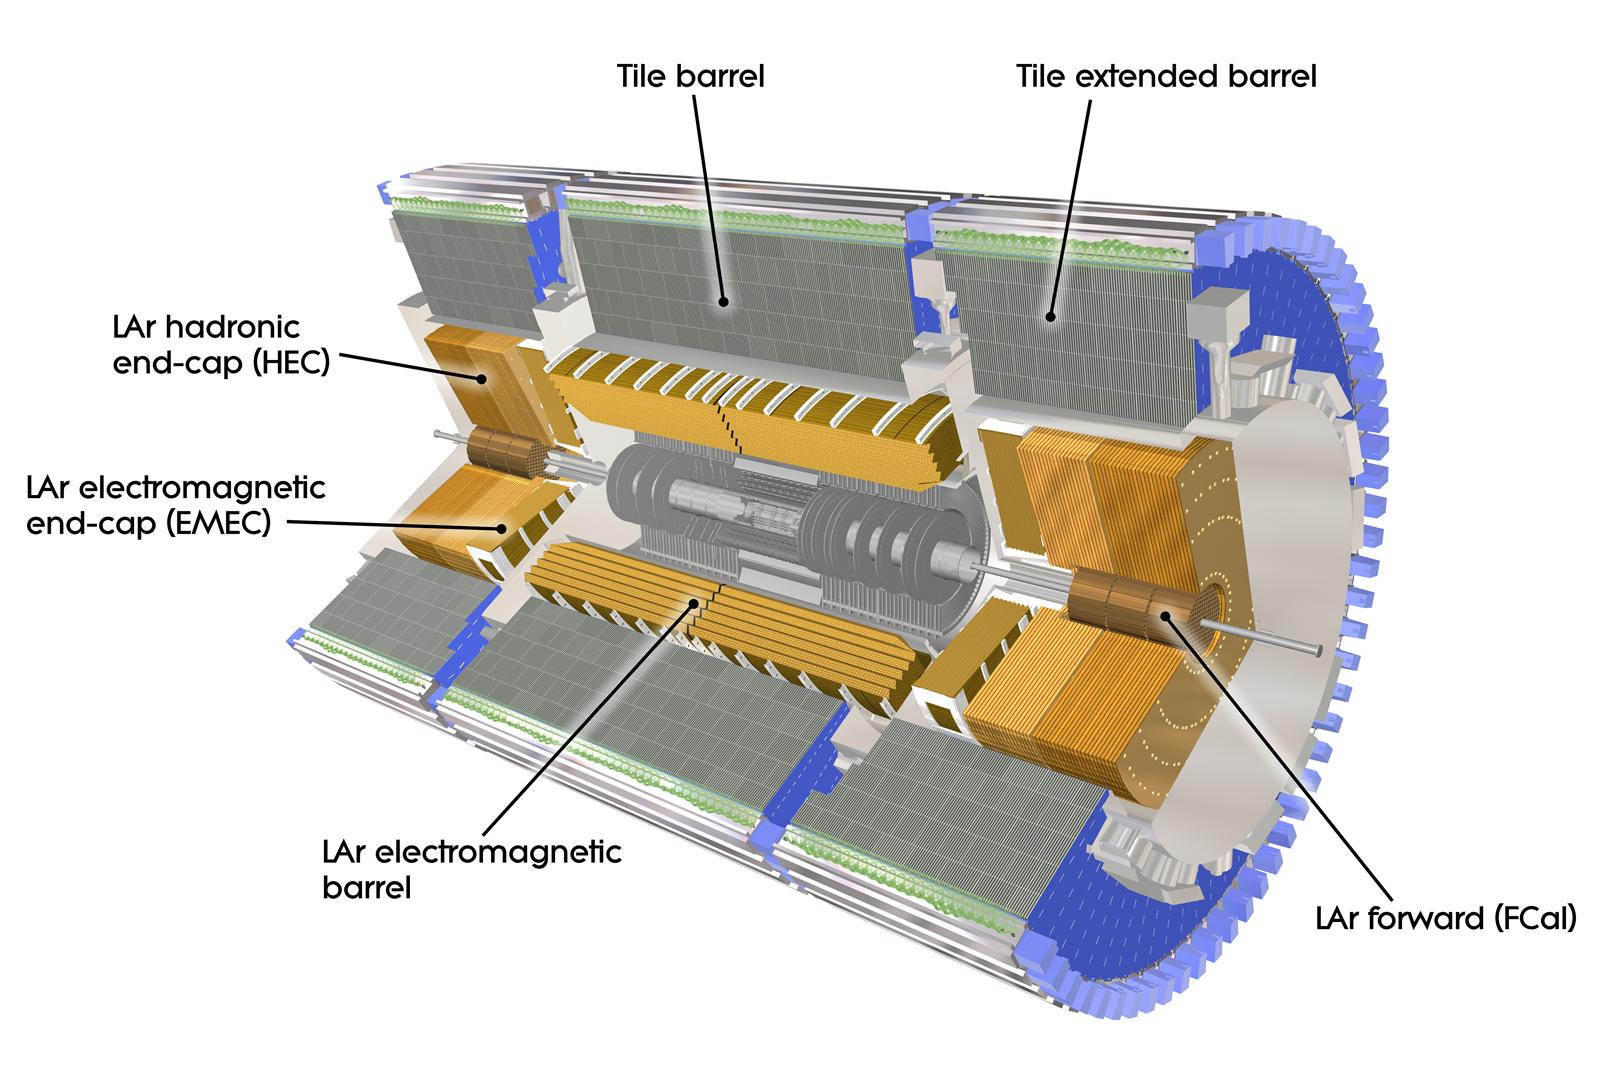
\includegraphics[width=.98\linewidth]{figures/LHC/ATLAS_CALO.jpeg}
    \caption{ A schematic of electromagnetic and hadronic calorimeters In ATLAS \cite{ATLAS}.\label{fig:ATLAS_Cals}}
\end{figure}

\subsection{Muon Spectrometer}
\label{subsec:MS}
In ATLAS, muons are deeply-penetrating charged particles that leave minimum ionizing deposits in the calorimeter. The muon spectrometer, the outermost part of the ATLAS detector, tracks muon trajectories giving an additional measure of muon's momentum that is deflected in $0.5$ magnetic field provided by the superconducting toroidal magnets \cite{ATLAS}. The MS tracks muon with $p_{T} > 3$ GeV in $|\eta| < 2.7$ range \cite{ATLAS}. As shown in figure \ref{fig:ATLAS_MS}, the muon spectrometer comprises four types of detectors; first, the three stations of Monitored Drift Tubes (MDT) in $|\eta| < 2.0$ region followed by the Cathode Strip Chambers (CSC) in  $2.0 < |\eta| < 2.7$ region \cite{ATLAS}. The other two detectors are the Resistive Plate Chambers (RPC) in $|\eta| < 1.05$ and the Thin-gap Chambers (TGC) beyond $|\eta| = 1.05$ comprising the trigger system in MS \cite{ATLAS}. 

\begin{figure}
    \centering
    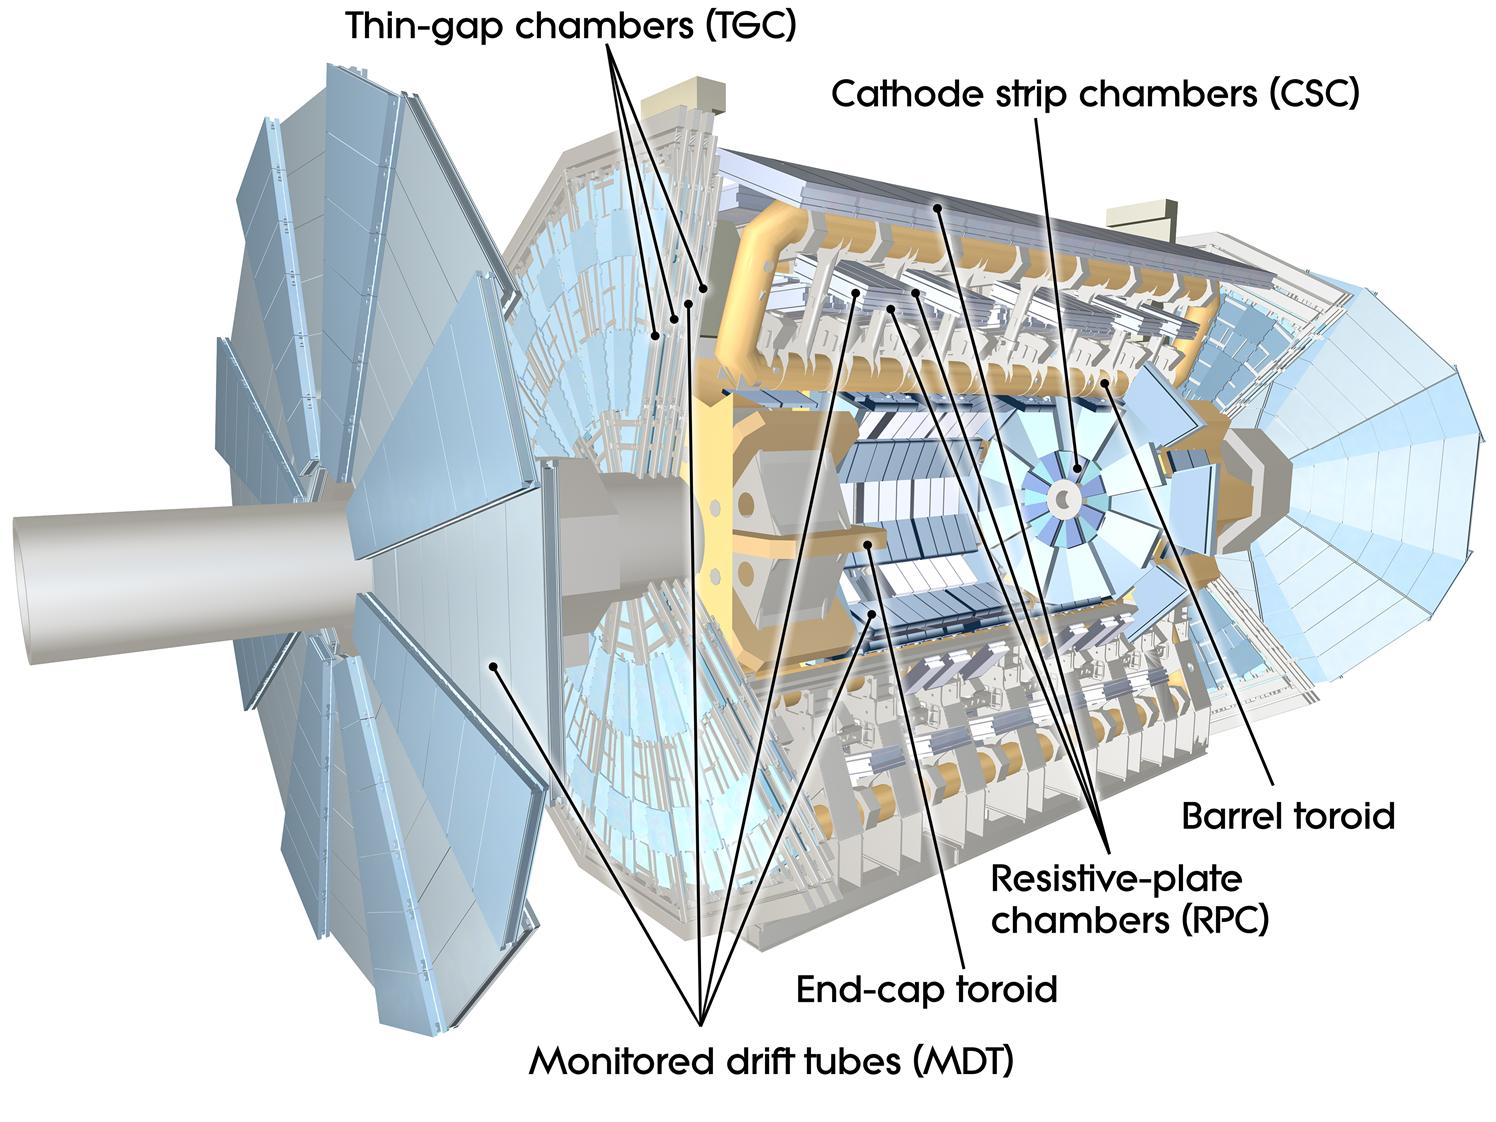
\includegraphics[width=.98\linewidth]{figures/LHC/ATLAS_MS.jpeg}
    \caption{ A schematic of different components of the muon spectrometer in ATLAS \cite{ATLAS}.\label{fig:ATLAS_MS}}
\end{figure}